% Figura: estratégias de transferência do modelo proposto (partes congeladas x treináveis).
%
% Uso no artigo (template IEEE, uma coluna):
%   no preâmbulo:  \usepackage[brazil]{babel}  (para a legenda sair "Figura")
%                  \usepackage{amsmath,amssymb}
%                  \usepackage{tikz}
%                  \usetikzlibrary{arrows.meta,patterns,positioning}
%   no texto:      copie o bloco \begin{figure}...\end{figure} abaixo.
%
% Este arquivo também compila sozinho (pdflatex modelo_proposto.tex) para conferir o desenho.
\documentclass[10pt]{article}
\usepackage[a4paper,textwidth=3.5in]{geometry} % largura de uma coluna IEEE
\usepackage[utf8]{inputenc}
\usepackage[T1]{fontenc}
\renewcommand{\figurename}{Figura} % no artigo, \usepackage[brazil]{babel} faz isso
\usepackage{amsmath,amssymb}
\usepackage{tikz}
\usetikzlibrary{arrows.meta,patterns,positioning}
\begin{document}

% ======================= início do bloco para o artigo =======================
\begin{figure}[t]
\centering
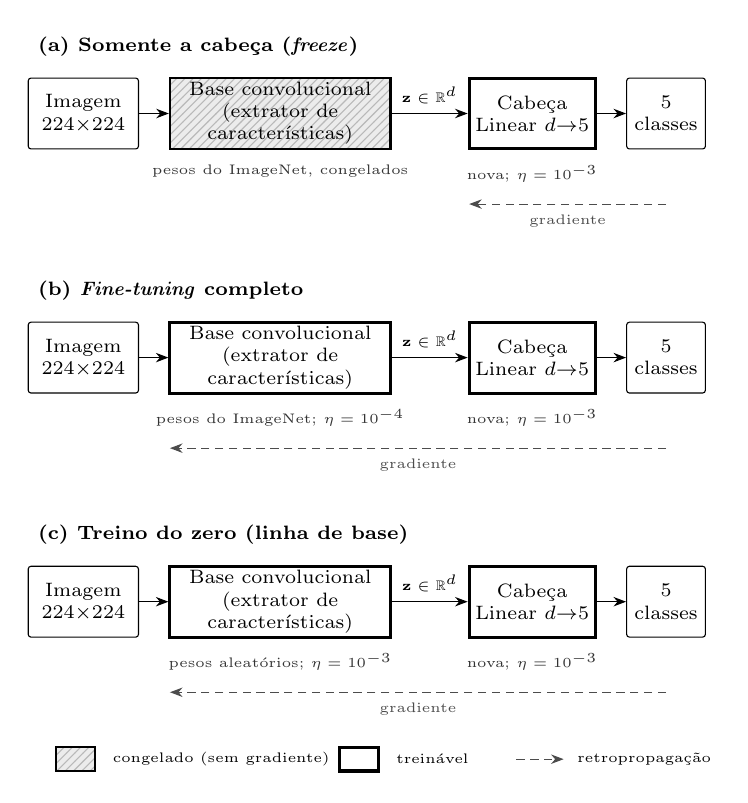
\begin{tikzpicture}[
    x=1mm, y=1mm,
    font=\scriptsize,
    >={Stealth[length=1.6mm]},
    bloco/.style={draw, thick, align=center, inner sep=1pt},
    congelado/.style={bloco, preaction={fill=gray!15}, pattern=north east lines, pattern color=gray!55},
    treinavel/.style={bloco, fill=white, line width=1.1pt},
    neutro/.style={draw, align=center, inner sep=1pt, rounded corners=1pt},
    nota/.style={font=\tiny, align=center, text=black!80},
    retro/.style={densely dashed, ->, black!70},
]
% ---------------------------------------------------------------------------
% Uma linha por estratégia: \linha{y}{título}{estilo da base}{nota da base}{até onde chega o gradiente}
\newcommand{\linha}[5]{
    \node[anchor=west, font=\scriptsize\bfseries] at (0, #1+8.5) {#2};
    % blocos
    \node[neutro, minimum width=14mm, minimum height=9mm] (in)  at (7,  #1) {Imagem\\$224{\times}224$};
    \node[#3,     minimum width=28mm, minimum height=9mm] (bb)  at (32, #1) {Base convolucional\\(extrator de\\características)};
    \node[treinavel, minimum width=16mm, minimum height=9mm] (hd) at (64, #1) {Cabeça\\Linear $d{\to}5$};
    \node[neutro, minimum width=10mm, minimum height=9mm] (out) at (81, #1) {5\\classes};
    % fluxo direto
    \draw[->] (in) -- (bb);
    \draw[->] (bb) -- node[above, font=\tiny] {$\mathbf{z}\in\mathbb{R}^{d}$} (hd);
    \draw[->] (hd) -- (out);
    % notas sob os blocos
    \node[nota, below=0.6mm of bb] {#4};
    \node[nota, below=0.6mm of hd] {nova; $\eta=10^{-3}$};
    % retropropagação: do erro até onde há parâmetros treináveis
    \draw[retro] (81, #1-11.5) -- (#5, #1-11.5)
        node[pos=0.5, below=0.1mm, font=\tiny, text=black!70] {gradiente};
}
% ---------------------------------------------------------------------------
\linha{0}{(a) Somente a cabeça (\textit{freeze})}{congelado}{pesos do ImageNet, congelados}{56}
\linha{-31}{(b) \textit{Fine-tuning} completo}{treinavel}{pesos do ImageNet; $\eta=10^{-4}$}{18}
\linha{-62}{(c) Treino do zero (linha de base)}{treinavel}{pesos aleatórios; $\eta=10^{-3}$}{18}

% legenda
\node[congelado, minimum width=5mm, minimum height=3mm] (lc) at (6, -82) {};
\node[anchor=west, font=\tiny] at (9.5, -82) {congelado (sem gradiente)};
\node[treinavel, minimum width=5mm, minimum height=3mm] (lt) at (42, -82) {};
\node[anchor=west, font=\tiny] at (45.5, -82) {treinável};
\draw[retro] (62, -82) -- (68, -82);
\node[anchor=west, font=\tiny] at (68.5, -82) {retropropagação};
\end{tikzpicture}
\caption{Estratégias de transferência avaliadas. Em todas, a camada de classificação original
(1000 classes do ImageNet) é substituída por uma camada linear nova com 5 saídas, e a entrada é
redimensionada e normalizada como no pré-treino. Em (a) apenas a cabeça recebe gradiente; em (b) a
base também é ajustada, com taxa de aprendizado $\eta$ dez vezes menor; em (c) a mesma arquitetura
parte de pesos aleatórios. A dimensão $d$ do vetor de características depende da arquitetura:
512 (ResNet-18), 2048 (ResNet-50), 1280 (EfficientNet-B0 e MobileNetV3-Large) e 768 (ConvNeXt-Tiny).}
\label{fig:modelo_proposto}
\end{figure}
% ======================== fim do bloco para o artigo ========================

\end{document}
